\begin{figure}[H]
\centering
\resizebox{0.25\textwidth}{!}{
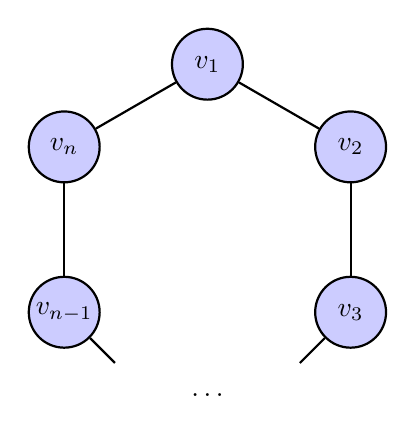
\begin{tikzpicture}[
  scale=0.7,
  vnode/.style={circle, fill=blue!20, draw=black, thick, inner sep=0pt, minimum size=0.9cm}
]

  % Vértices iniciales (lado derecho)
  \node[vnode] (v1) at (90:3) {$v_1$};
  \node[vnode] (v2) at (30:3) {$v_2$};
  \node[vnode] (v3) at (-30:3) {$v_3$};

  % Vértices finales (lado izquierdo)
  \node[vnode] (vn1) at (210:3) {$v_{n-1}$};
  \node[vnode] (vn) at (150:3) {$v_n$};

  % Puntos suspensivos y nodos auxiliares para continuar las aristas en la parte inferior
  \node[draw=none, fill=none] (dots) at (-90:3) {$\dots$};
  \node[draw=none, fill=none, minimum size=0pt] (v3_inv) at (-60:3) {};
  \node[draw=none, fill=none, minimum size=0pt] (vn1_inv) at (-120:3) {};

  % Aristas continuas visibles
  \draw[thick] (v1) -- (v2);
  \draw[thick] (v2) -- (v3);
  \draw[thick] (vn1) -- (vn);
  \draw[thick] (vn) -- (v1); % Arista que cierra el ciclo entre v_n y v_1

  % Aristas que se dirigen hacia la elipsis inferior
  \draw[thick] (v3) -- (v3_inv);
  \draw[thick] (vn1_inv) -- (vn1);

\end{tikzpicture}}
\caption{El grafo $C^n$}
\label{fig:ciclo_n}
\end{figure}
